% !TeX root = ./../memoria.tex
\chapter{Diseño e implementación}

\definecolor{mygreen}{rgb}{0,0.6,0}
\definecolor{mygray}{rgb}{0.5,0.5,0.5}
\definecolor{mymauve}{rgb}{0.58,0,0.82}

%%%%%%%%%%%%%%%%%%%%%%%%%%%%%%%%%%%%%%%%%%%%%%%%%%%%%%%%%%%%%%%%%%%%%%%%%%%%%
% parámetros para configurar el formato del código en los entornos lstlisting
%%%%%%%%%%%%%%%%%%%%%%%%%%%%%%%%%%%%%%%%%%%%%%%%%%%%%%%%%%%%%%%%%%%%%%%%%%%%%
\lstset{ %
  backgroundcolor=\color{white},   % choose the background color; you must add \usepackage{color} or \usepackage{xcolor}
  basicstyle=\footnotesize,        % the size of the fonts that are used for the code
  breakatwhitespace=false,         % sets if automatic breaks should only happen at whitespace
  breaklines=true,                 % sets automatic line breaking
  captionpos=b,                    % sets the caption-position to bottom
  commentstyle=\color{mygreen},    % comment style
  deletekeywords={...},            % if you want to delete keywords from the given language
  %escapeinside={\%*}{*)},          % if you want to add LaTeX within your code
  %extendedchars=true,              % lets you use non-ASCII characters; for 8-bits encodings only, does not work with UTF-8
  %frame=single,	                % adds a frame around the code
  keepspaces=true,                 % keeps spaces in text, useful for keeping indentation of code (possibly needs columns=flexible)
  keywordstyle=\color{blue},       % keyword style
  language=C++,                % the language of the code
  %otherkeywords={*,...},           % if you want to add more keywords to the set
  numbers=left,                    % where to put the line-numbers; possible values are (none, left, right)
  numbersep=5pt,                   % how far the line-numbers are from the code
  numberstyle=\tiny\color{mygray}, % the style that is used for the line-numbers
  rulecolor=\color{black},         % if not set, the frame-color may be changed on line-breaks within not-black text (e.g. comments (green here))
  showspaces=false,                % show spaces everywhere adding particular underscores; it overrides 'showstringspaces'
  showstringspaces=false,          % underline spaces within strings only
  showtabs=false,                  % show tabs within strings adding particular underscores
  stepnumber=1,                    % the step between two line-numbers. If it's 1, each line will be numbered
  stringstyle=\color{mymauve},     % string literal style
  tabsize=2,	                   % sets default tabsize to 2 spaces
  title=\lstname,                  % show the filename of files included with \lstinputlisting; also try caption instead of title
  morecomment=[s]{/*}{*/}
}

\label{Capitulo3}

En este capítulo se exponen las decisiones de diseño tomadas para la construcción del robot propuesto. Se detallan las dimensiones de las piezas que constituyen el chasis, su esquema de conexiones eléctricas y finalmente la implementación del software y el firmware embebido para la navegación autónoma.

\section{Estructura mecánica}

En esta sección se describe la estructura física del robot y se explican los criterios utilizados tanto para el dimensionamiento de piezas como para su disposición.

\subsection{Disposición en niveles}
Tal como se menciona en la sección \ref{sec:turtlebot}, el diseño propuesto toma como referencia a la base móvil \textit{open source} Turtlebot 2. Por este motivo, LuboBot también se compone de una base móvil cilíndrica de tracción diferencial que funciona como soporte para una estructura escalable en "niveles", gracias a lo que el usuario puede agregar nuevos componentes sin dificultad, según los requisitos particulares de su aplicación. En la figura \ref{fig:lubobotURDF} y \ref{fig:lubobotReal} muestran respectivamente una representación en 3D de la estructura física del robot y una fotografía de su montaje real.

\begin{figure}[ht]
  \centering
  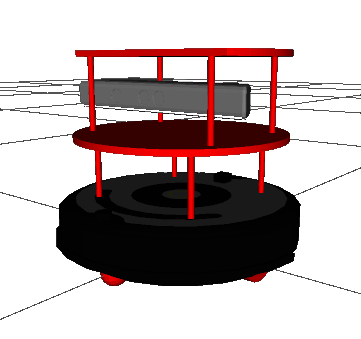
\includegraphics[scale=0.5]{./Figures/lubobot_urdf.png}
  \caption{Vista frontal del modelo URDF de LuboBot representado en RViz.}
  \label{fig:lubobotURDF}
\end{figure}

\begin{figure}[ht]
  \centering
  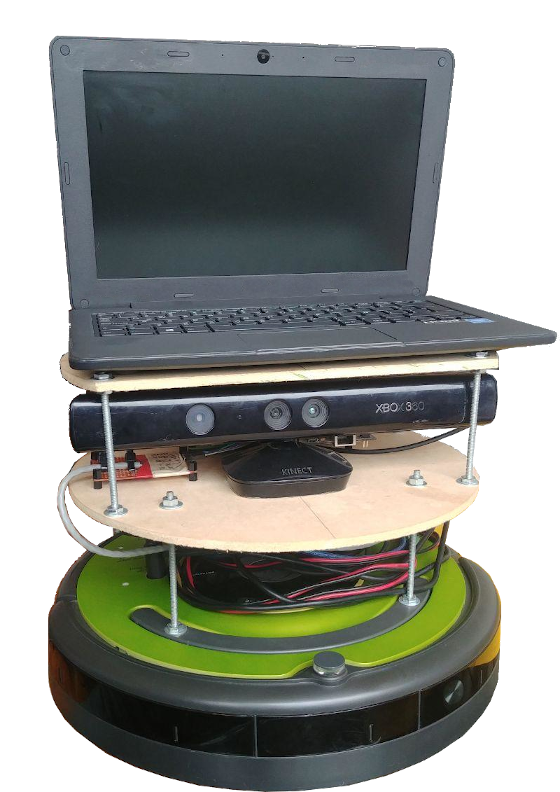
\includegraphics[scale=0.5]{./Figures/lubobot.png}
  \caption{Fotografía frontal del montaje del robot LuboBot.}
  \label{fig:lubobotReal}
\end{figure}

\newpage

Sobre la base móvil se montaron cuatro varillas roscadas de 5 mm de diámetro y 80 mm de largo, de las cuales las dos frontales fueron fijadas a la agarradera o  \textit{handler} del Roomba, mientras que las dos traseras se fijaron directamente al chasis. Dicha disposición fue calculada en base a las áreas del robot que el autor determinó como seguras para su modificación, es decir que no representaban ningún riesgo al correcto funcionamiento de la base móvil.

\subsection{Disposición de componentes}

Los diferentes componentes funcionales del robot fueron dispuestos en la configuración que se aprecia en la figura \ref{fig:lubobotComponentes}, a excepción de la \textit{laptop}, presente solo para fines de ejemplo ya que no forma parte del robot. Para la disposición propuesta se tuvieron en cuenta los siguientes criterios:

\begin{itemize}
  \item Mantener bajo el centro de gravedad del conjunto.
  \item Maximizar el espacio libre en el nivel superior para futuros \textit{upgrades}.
  \item Posicionar la IMU lo más cerca posible del centro de rotación de la base y lo más abajo posible.
  \item Posicionar el sensor Kinect a alrededor de 30 cm del suelo para incrementar su línea de visión.
  \item Mantener libre de obstrucciones el acceso al botón central del Roomba.
\end{itemize}

\begin{figure}[ht]
  \centering
  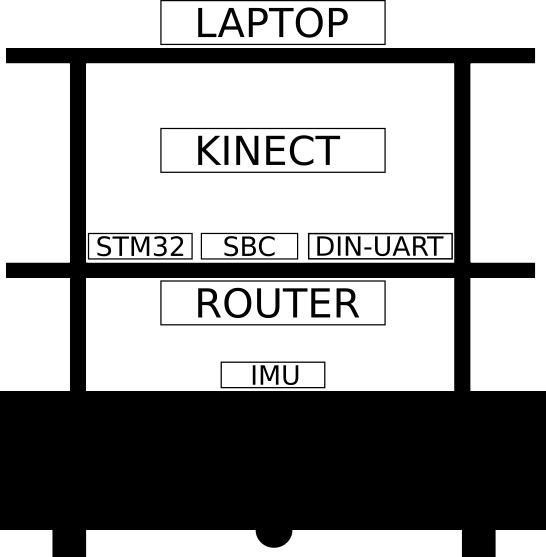
\includegraphics[scale=0.4]{./Figures/distribucion_componentes.png}
  \caption{Distribución de componentes del robot.}
  \label{fig:lubobotComponentes}
\end{figure}

\section{Diagrama en bloques de conexiones}

En la figura \ref{fig:lubobotConexiones} se muestra el diagrama de conexiones entre los distintos componentes electrónicos del sistema y se indica además el protocolo utilizado para cada interacción. Se decidió dotar al robot de un \textit{router} Wifi a bordo a modo de facilitar su conexión a una computadora externa, destinada como estación de control para el envío de misiones.

\begin{figure}[ht]
  \centering
  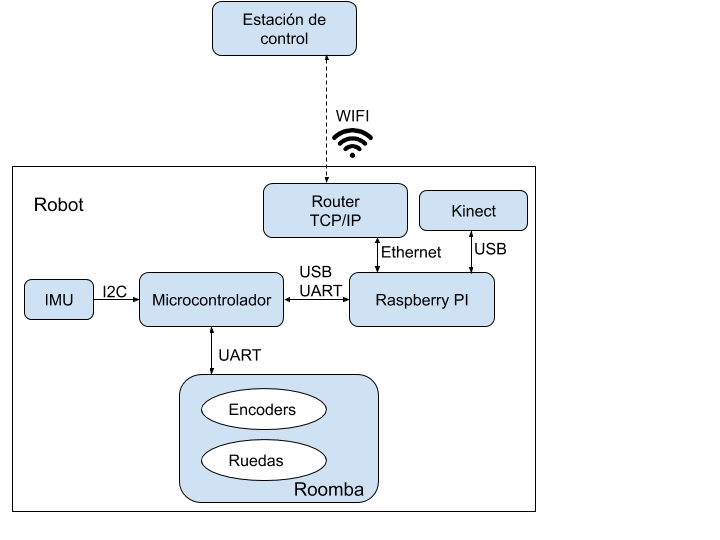
\includegraphics[scale=0.5]{./Figures/lubobot_conexiones.png}
  \caption{Diagrama de conexiones de los componentes constitutivos del robot.}
  \label{fig:lubobotConexiones}
\end{figure}

\newpage

\section{Implementación de firmware}

En esta sección se detallan las decisiones de diseño e implementación del firmware, encargado de la interconexión del robot Roomba y la Raspberry PI así como también de la lectura de sensores ajenos a la base móvil original como la IMU.

\subsection{Distribución de tareas en FreeRTOS}

Debido a la necesidad de atender rutinas de naturaleza tanto síncrona como asíncrona en el firmware, se decidió utilizar un RTOS para su implementación. Las tareas involucradas se describen a continuación, agrupadas en base a su responsabilidad dentro del sistema.

\subsection{Interfaz Roomba-microcontrolador}

La interfaz Roomba-microcontrolador se conforma por dos tareas que en conjunto cumplen la función de \textit{proxy} entre la base móvil Roomba y el resto del sistema. El microcontrolador se ocupa de la serialización y des-serialización de los paquetes intercambiados con el robot mediante el protocolo Open Interface. Las tareas responsables del manejo de esta función se describen a continuación.

\begin{itemize}
  \item Solicitud de lectura de sensores: realiza la lectura de cada uno de los dos encoders disponibles de manera periódica cada 100 ms y actualiza las variables internas de estado en cada iteración con el valor actualizado.
  \item Envío de comandos a actuadores: realiza el despacho de comandos a los distintos actuadores disponibles en base a las órdenes recibidas desde ROS. Si bien esta tarea puede considerarse de carácter asíncrono, se implementó sobre esta un mecanismo de \textit{watchdog} para evitar que un posible fallo en la comunicación con ROS ponga en peligro la integridad del usuario y del robot. Para esto, la tarea verifica cada 100 ms la existencia de un comando de velocidad nuevo. En su ausencia, envía una orden para detener el robot.
\end{itemize}

Se escribió una biblioteca en lenguaje C++ bajo el nombre de ``Roomba600'' que ofrece una interfaz simplificada para la interacción del microcontrolador con el Roomba. Está implementada sobre la capa de abstracción STM32CubeHAL ofrecida por el fabricante ST, que permite el manejo de puertos serie UART con mecanismos de control asíncronos aptos para RTOS.

El protocolo Open Interface permite la interacción con todos los sensores y actuadores disponibles en el robot Roomba. Sin embargo, los requerimientos del presente proyecto se limitan al control de velocidad de ruedas y lectura de encoders, por lo que en la biblioteca presentada se implementan solamente las interfaces para dichas funciones y se dejan los demás métodos pendientes de implementación para un trabajo futuro. En el código \ref{cod:Roomba600} se muestra la interfaz de la clase Roomba600 con los métodos actualmente implementados.


\begin{lstlisting}[label=cod:Roomba600,caption=Interfaz de la clase Roomba600 que implementa el protocolo Open Interface\protect\footnotemark.]
class Roomba600 {
public:
	/// @brief Constructs Roomba600 object with given parameters
	/// @param _uart pointer to the STM32CubeHAL UART handler
	/// @param _brcPort pointer to the STM32CubeHAL BRC port
	/// @param _brcPin pointer to the STM32CubeHAL BRC pin
	Roomba600(UART_HandleTypeDef *_uart, GPIO_TypeDef *_brcPort,
      uint16_t _brcPin);
	/// @brief Initializes data stream.
	void start();
	/// @brief Resets communication.
	void reset();
	/// @brief Stops robot and data stream.
	void stop();
	/// @brief Switches to safe mode.
	void goSafeMode();
	/// @brief Switches to full mode (be careful).
	void goFullMode();
	/// @brief Switches to passive mode.
	void goPassiveMode();
  /// @brief Sets independent velocity set-points for each wheel in m/s.
  /// Relies on internal PID loop from the Roomba.
	void driveVelocity(int16_t leftVel, int16_t rightVel);
	/// @brief Sets independent PWM values to each wheel.
  void drivePWM(int16_t leftPWM, int16_t rightPWM);
	/// @brief Pauses the stream of sensor data reads.
	void pauseStream();
	/// @brief Resumes the stream of sensor data reads.
	void resumeSteam();
	/// @brief Retrieves left encoder value.
	uint16_t readLeftEncoder();
	/// @brief Retrieves right encoder value.
  uint16_t readRightEncoder();
}
\end{lstlisting}

\footnotetext{Definición de la clase en el repositorio del proyecto \url{https://github.com/apojomovsky/lubobot/blob/master/firmware/proyecto_unificado/create_2/Inc/create2.h}}

\subsection{Interfaz microcontrolador-ROS}

La interfaz entre el microcontrolador y ROS requirió de la migración de la biblioteca rosserial, mencionada en la sección \ref{sec:rosserial}. Esta biblioteca hace posible entablar una comunicación serial asíncrona entre el microcontrolador y una computadora con ROS mediante un protocolo que utiliza los mensajes estándares de ROS. A nivel del microcontrolador se optó por implementar esta interfaz mediante tres tareas que se describen a continuación:

\begin{itemize}
  \item Spin de ROS: esta tarea se encarga de llamar al método spin de la biblioteca rosserial de manera periódica. Cumple la función de \textit{heartbeat} para la comunicación con la computadora, por la que ambas partes se indican mutuamente si existen mensajes o servicios que transmitir.
  \item Suscriptor de ROS: recibe los mensajes y solicitudes de servicios que fueron enviados desde ROS al microcontrolador y llama a las funciones de \textit{callback} requeridas para cada uno de ellos.
  \item Publicador de ROS: despacha los mensajes y solicitudes de servicios que salen del microcontrolador.
\end{itemize}

Para la migración de la biblioteca rosserial fue necesario implementar una clase cuyas interfaces fueran compatibles con la definición mostrada en el código \ref{cod:stm32hardware}.

\begin{lstlisting}[label=cod:stm32hardware, caption=Interfaz de la clase STM32Hardware requerida por la biblioteca rosserial\protect\footnotemark.]

class STM32Hardware {
  public:
	  /// @brief Constructs STM32Hardware object with given parameter
	  /// @param huart_ pointer to the STM32CubeHAL UART handler
    STM32Hardware(UART_HandleTypeDef *huart_);
	  /// @brief Initializes comunication.
    void init();
	  /// @brief Reads from input buffer.
    int read();
	  /// @brief Writes data of a given length.
	  /// @param data pointer to bytes array.
	  /// @param length number of bytes to transmit.
    void write(uint8_t* data, int length);
	  /// @brief Returns time elapsed since startup in milliseconds.
    unsigned long time();
};

\end{lstlisting}

\footnotetext{Clase STM32Hardware implementada en el proyecto \url{https://github.com/apojomovsky/lubobot/blob/master/firmware/proyecto_unificado/ros_lib/STM32Hardware.h}}

\section{Implementación de software}

En esta sección se detalla la organización del código y archivos que acompañan al robot propuesto en este trabajo.

\subsection{Metapaquete LuboBot para ROS}

En esta sección se explica la estructura del meta-paquete LuboBot, que contiene las herramientas mínimas necesarias para comandar, modificar e inspeccionar el robot con ROS.

Como se describió en la sección \ref{sec:organizacionArchivos}, se considera una buena práctica el utilizar un metapaquete para contener varios paquetes que estan relacionados entre sí. Siguiendo estas recomendaciones, el software que acompaña al robot propuesto se organiza de la siguiente manera:

\begin{itemize}
  \item lubobot\_description: incluye los archivos de descripción del robot en formato URDF y los archivos de visualización para RViz.
  \item lubobot\_msgs: incluye los mensajes utilizados para intercambiar información entre el firmware y ROS, a través de rosserial.
  \item lubobot\_drivers: incluye el código de fuente para los nodos o programas que monitorean los sensores del robot, así como los que envían comandos a los actuadores.
\end{itemize}

\subsection{Nodo re-publicador de IMU ``lubo\_imu\_relay''}

Se encuentra suscripto a los mensajes del tipo lubo\_imu, compuesto por las lecturas crudas de orientación y aceleración angular provenientes del microcontrolador. El programa se encarga de procesarlos a medida que llegan, agregándoles información de tiempo y secuencia y luego los republica en el formato de mensaje estándar de ROS para unidades de medición inercial\protect\footnotemark.

\footnotetext{Definición de mensaje estándar de ROS para Imu \url{http://docs.ros.org/kinetic/api/sensor_msgs/html/msg/Imu.html}}

Cabe preguntarse por qué no evitar este nodo y publicar mensajes con el tipo estándar directamente desde el microcontrolador. Hay dos motivos específicos que son válidos no solo para este mensaje en particular, sino también para la gran mayoría de los mensajes intercambiados con el microcontrolador:
\begin{itemize}
  \item los mensajes estandar de ROS poseen un \textit{footprint} en memoria poco adecuado para dispositivos con poca memoria RAM.
  \item el bus UART utilizado para la comunicación con el microcontrolador ofrece un ancho de banda ajustado que se satura rápidamente con mensajes del tipo estándar.
\end{itemize}

Las unidades de medición inercial precisan ser calibradas antes de utilizarse, esto permite compensar el sesgo o \textit{bias} inherente a cada sensor. Esta calibración se realiza en el microcontrolador como parte de la rutina de inicialización, por lo que para el nodo aquí descripto se asume que la IMU ya se encuentra calibrada.

\subsection{Nodo publicador de odometría ``lubo\_odom\_node''}

Está suscripto a los mensajes del tipo lubo\_encoders que provienen del microcontrolador. El mensaje se compone de las lecturas de los encoders izquierdo y derecho de la base Roomba. Cabe mencionar que las lecturas de ambos encoders deben tomarse en simultáneo para el correcto cálculo de la odometría, es por esto que el mensaje utilizado incluye ambas lecturas.

El microcontrolador publica los mensajes a una frecuencia por defecto de 20 Hz, pero este y otros parámetros son también configurables desde la estación de control en \textit{runtime}. Esto se logra gracias al mecanismo de configuración rosparam, que ahorra la necesidad de recompilar el código cada vez que se deba actualizar algún parámetro.

\subsection{Configuración del paquete ros\_localization}

Así como se describió en la subsección \ref{sec:robotLocalization}, es necesario definir una matriz de booleanos para cada uno de los sensores o fuentes de información que consume el estimador. Para el presente trabajo, se utilizaron las mediciones provistas por dos fuentes distintas:

\begin{itemize}
  \item unidad de medición inercial.
  \item odometría generada a partir encoders.
\end{itemize}

Para la configuración del paquete se utilizó un archivo del tipo YAML que se carga de manera automática al servidor de parámetros de ROS al inicio de cada ejecución. Las partes más importantes de este archivo residen en la configuración de campos a ser tomados en cuenta por el estimador para cada una de las fuentes de información. Una versión reducida de esta configuración se muestra en el bloque de código \ref{cod:rosLocalization}.

\newpage

\newcommand\YAMLcolonstyle{\color{green}\mdseries}
\newcommand\YAMLkeystyle{\color{black}\bfseries}
\newcommand\YAMLvaluestyle{\color{blue}\mdseries}

\makeatletter

% here is a macro expanding to the name of the language
% (handy if you decide to change it further down the road)
\newcommand\language@yaml{yaml}

\expandafter\expandafter\expandafter\lstdefinelanguage
\expandafter{\language@yaml}
{
keywords={true,false,null,y,n},
keywordstyle=\color{darkgray}\bfseries,
basicstyle=\YAMLkeystyle,                                 % assuming a key comes first
sensitive=false,
comment=[l]{\#},
morecomment=[s]{/*}{*/},
commentstyle=\color{mygreen}\ttfamily,
stringstyle=\YAMLvaluestyle\ttfamily,
moredelim=[l][\color{orange}]{\&},
moredelim=[l][\color{magenta}]{*},
moredelim=**[il][\YAMLcolonstyle{:}\YAMLvaluestyle]{:},   % switch to value style at :
morestring=[b]',
morestring=[b]",
literate =    {---}{{\ProcessThreeDashes}}3
{>}{{\textcolor{red}\textgreater}}1
{|}{{\textcolor{red}\textbar}}1
{\ -\ }{{\mdseries\ -\ }}3,
}

% switch to key style at EOL
\lst@AddToHook{EveryLine}{\ifx\lst@language\language@yaml\YAMLkeystyle\fi}
\makeatother

\newcommand\ProcessThreeDashes{\llap{\color{cyan}\mdseries-{-}-}}

\begin{lstlisting}[language=yaml, label=cod:rosLocalization, caption=Configuraciones del filtro proveído por el paquete ros\_localization \protect\footnotemark.]

# Odometry configuration
odom_frame: odom
base_link_frame: base_link

# Input topic name for odometry
odom0: /odom

# For the odometry source, we only consider vx, vy and vyaw
odom0_config: [false, false, false,
               false, false, false,
               true,  true,  false,
               false, false, true,
               false, false, false]

# IMU configuration

# Input topic name for IMU
imu0: /imu/data_raw

# For the IMU source we consider only yaw, vyaw and ax
imu0_config: [false, false, false,
              false, false, true,
              false, false, false,
              false, false, true,
              true, false, false]

\end{lstlisting}

\footnotetext{Archivo de configuración YAML completo \url{https://github.com/apojomovsky/lubobot/blob/master/lubobot/config/ekf.yaml}}

% TODO
% \subsection{Configuración del paquete move\_base}\label{sec:move_base}
% \subsection{Configuración del paquete amcl}\label{sec:amcl}

\section{Herramientas ofrecidas al usuario}

De acuerdo a los objetivos del presente trabajo, el desarrollo del robot móvil LuboBot está acompañado de una serie de herramientas y documentos con los que se pretende facilitar el proceso de adopción de la plataforma por nuevos usuarios.

\subsection{Entorno de desarrollo encapsulado}

La instalación de un entorno de desarrollo compatible con un proyecto puede tornarse una tarea muy frustrante para el usuario si no se toman los recaudos necesarios. Casos como el del uso de un sistema operativo total o parcialmente incompatible, diferencias de versiones de las bibliotecas requeridas e instaladas, son solo algunos de los problemas con los que el usuario promedio podría encontrarse.

Con la intención de simplificar al máximo el proceso de instalación de dependencias, se provee un entorno de desarrollo encapsulado utilizando la tecnología de \textit{containers} mediante la plataforma Docker\protect\footnotemark.

\footnotetext{Página web del proyecto Docker \url{https://www.docker.com}}

Esta utilidad permite la generación de entornos de trabajo aislados del sistema operativo \textit{host} mediante el uso de un archivo especial denominado Dockerfile, en el que se detalla una lista de acciones a seguir para generar el entorno de trabajo. En el presente trabajo, se incluyen los siguientes archivos:


\begin{itemize}
  \item \textbf{Dockerfile}: continene las definiciones para generar el entorno de trabajo con todas las dependencias necesarias para la ejecución del software del robot en ROS.
  \item \textbf{build\_docker.sh}: \textit{script} encargado de generar el entorno de desarrollo, solo es necesario ejecutarlo una única vez.
  \item \textbf{run\_docker.sh}: \textit{script} encargado de lanzar el entorno de desarrollo. El usuario deberá llamarlo cada vez que desee arrancar el sistema.
\end{itemize}


Se proveen instrucciones específicas sobre cómo utilizar y expandir la configuración inicial propuesta de esta herramienta en la Wiki del proyecto.

\subsection{Documentación en formato Wiki}

Se ofrece en conjunto con el repositorio Git\protect\footnotemark, una sección aparte dedicada exclusivamente a la documentación del robot. Para este fin se utilizó la funcionalidad de \textit{Wiki} ofrecida por la plataforma Github.

\footnotetext{Repositorio principal del proyecto LuboBot \url{https://github.com/apojomovsky/lubobot}}


En la figura \ref{fig:wiki} se muestra la página principal de la Wiki en su primera iteración, donde se realiza una breve presentación del proyecto, seguida de \textit{links} de interés con tutoriales y especificaciones técnicas.

Se decidió utilizar este formato de documentación en favor de incluir todo en el archivo \file{README.md} por una suma de motivos entre los que se destacan:

\begin{itemize}
  \item organización de archivos en un sub-repositorio proveído de manera automática por Github, con historial de cambios separado del repositorio principal.
  \item estructura de archivos múltiples organizados en forma de árbol, que no solo facilitan la búsqueda de información por parte del usuario sino también las tareas de mantenimiento.
  \item generación automática de índice en forma de \textit{sidebar} en el sitio que facilita la navegación entre las páginas que lo componen.
\end{itemize}

\newpage

\begin{figure}[ht]
  \centering
  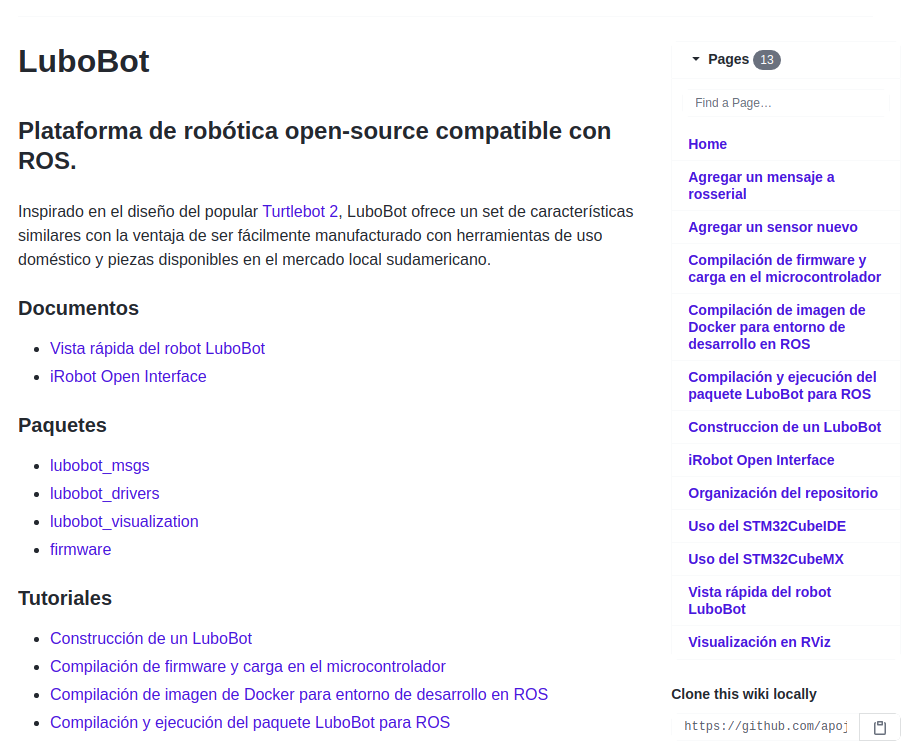
\includegraphics[scale=0.5]{./Figures/wiki.png}
  \caption{Página principal de la Wiki de LuboBot\protect\footnotemark.}
  \label{fig:wiki}
\end{figure}

\footnotetext{Wiki del proyecto LuboBot \url{https://github.com/apojomovsky/lubobot/wiki}}
